\section{Technical Appendix}
\label{app:technical}

\subsection{Code and reproduction}
\label{app:code}

The pipeline is a Python package (\texttt{aiprod}) in the project repository,
\begin{center}\url{https://github.com/samaypanwar/ai-substitute-or-complement}.\end{center}
The single command \texttt{python -m aiprod.run} downloads every source, builds the panels, estimates all models, and writes the figures and the tables included in this paper; no number in a table is entered by hand.

\subsection{Wild cluster bootstrap}

For a coefficient $\beta_k$ we fit the model with $\beta_k=0$ imposed, keep its fitted values $\tilde y$ and residuals $\tilde u$, and draw for each sector $g$ a weight $v_g$ from Webb's six-point distribution $\{\pm\sqrt{3/2}, \pm1, \pm\sqrt{1/2}\}$. Each bootstrap sample is $y^* = \tilde y + v_g \tilde u$; we refit the full model and record the cluster-robust $t$-statistic for $\beta_k$. The $p$-value is the share of 1,999 bootstrap $|t^*|$ at least as large as the observed $|t|$.

\subsection{Bayesian pooling}

With prior $\beta_{AI} \sim N(\hat\beta_{IT}, \mathrm{se}_{IT}^2+\tau^2)$ and likelihood $\hat\beta_{AI} \sim N(\beta_{AI}, \mathrm{se}_{AI}^2)$, the posterior mean is $w\hat\beta_{AI} + (1-w)\hat\beta_{IT}$ with $w = (\mathrm{se}_{IT}^2+\tau^2)/(\mathrm{se}_{IT}^2+\tau^2+\mathrm{se}_{AI}^2)$.

\subsection{Nowcast of the junior gap}
\label{app:nowcast}

The nowcast regresses the four-quarter change in each sector's QWI junior gap on sector fixed effects and the four-quarter changes in log sector employment (CES), the supervisory share of employment (CES), and the young-minus-prime unemployment gap (CPS ages 20--24 minus 25--54). It is fitted on 2001--2019 and evaluated on 2023Q1--2025Q3.

\begin{figure}[h]
  \centering
  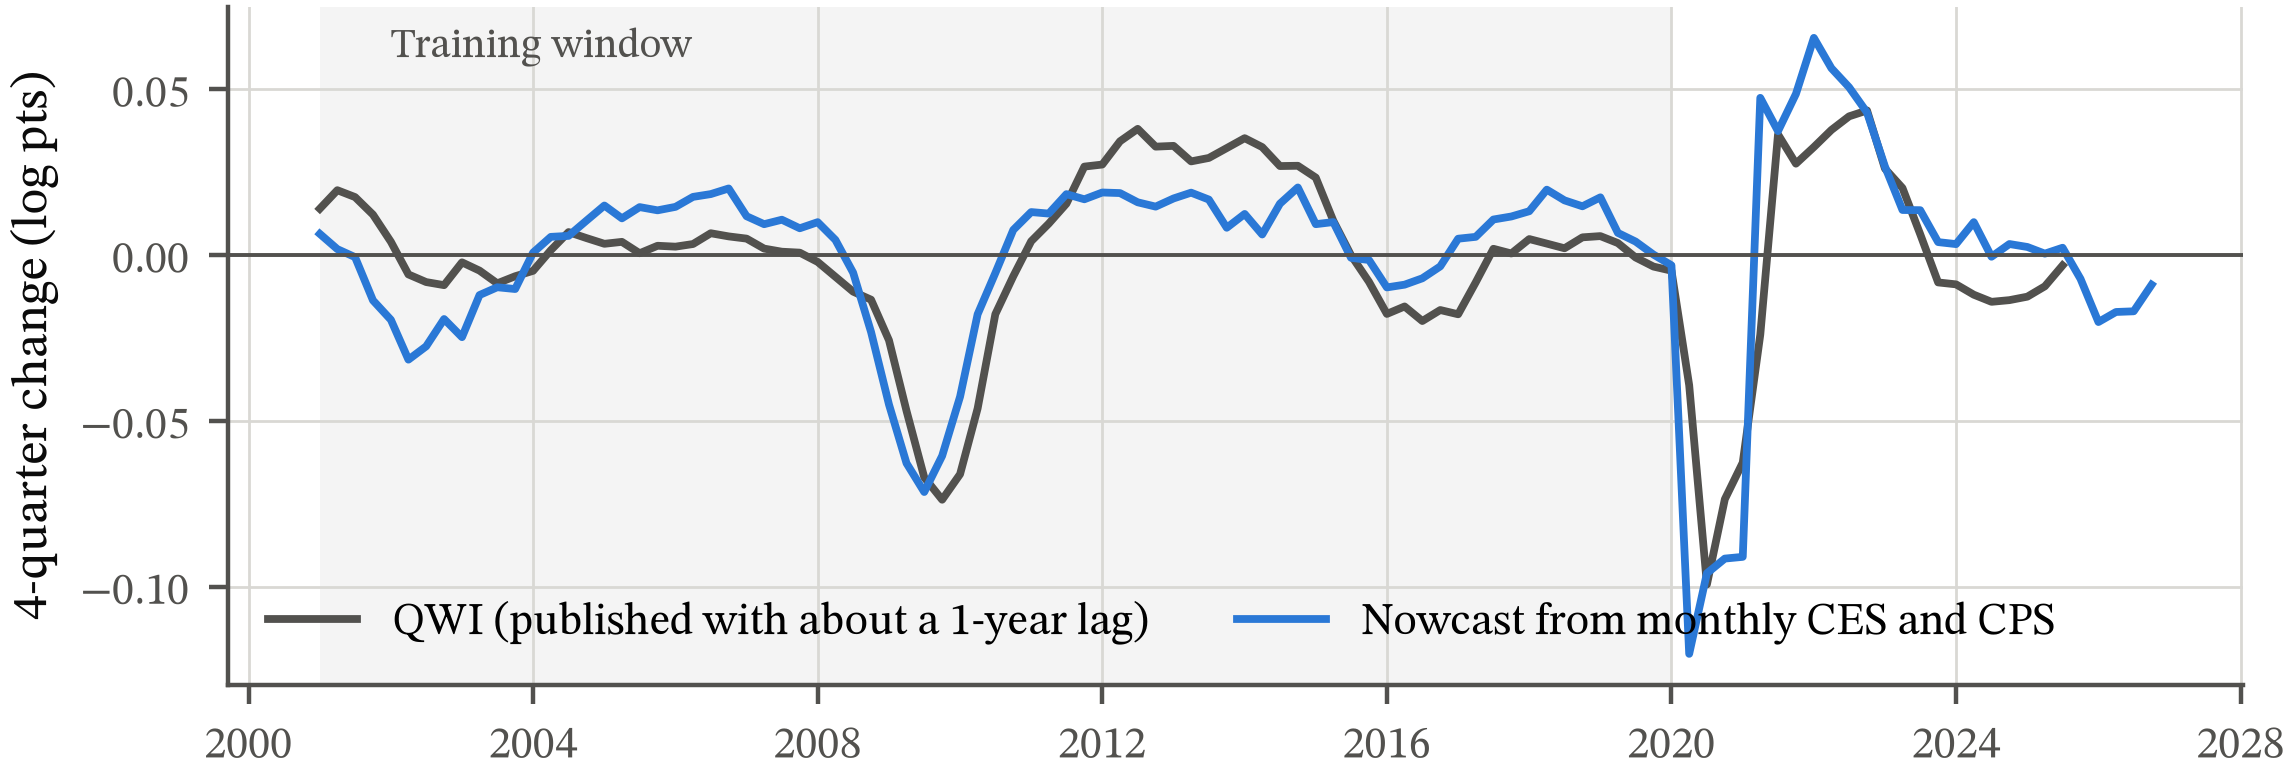
\includegraphics[width=\textwidth]{fig06_nowcast.png}
  \caption{Average four-quarter change in the junior employment gap across sectors: QWI as published (grey) and the nowcast from monthly data (blue). The shaded region is the training window; everything after 2019 is out of sample.}
  \label{fig:nowcast}
\end{figure}

\subsection{Additional figures}

\begin{figure}[h]
  \centering
  \begin{subfigure}[t]{0.49\textwidth}
    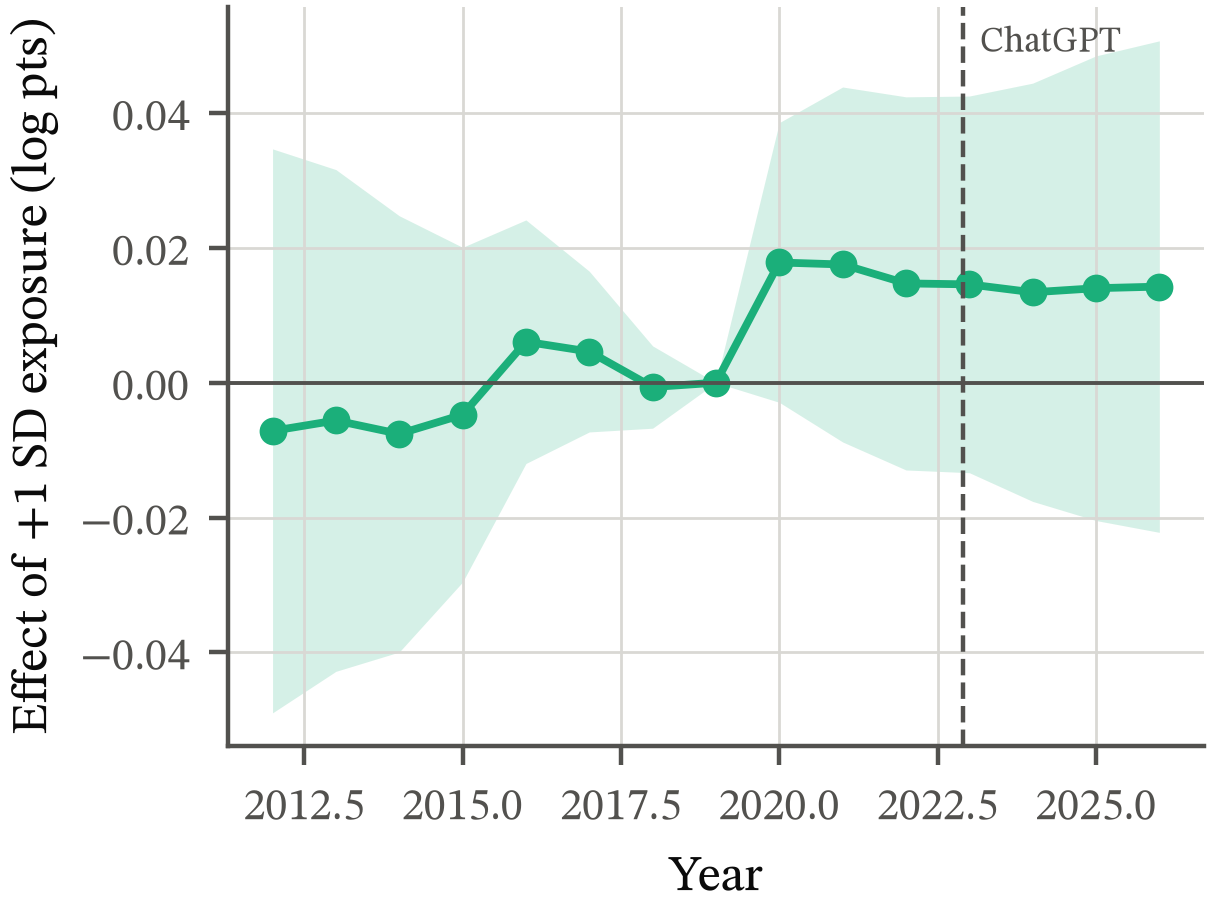
\includegraphics[width=\linewidth]{fig05_detailed_employment_event_study.png}
    \caption{Total employment, 91 detailed industries}
    \label{fig:detailed}
  \end{subfigure}\hfill
  \begin{subfigure}[t]{0.49\textwidth}
    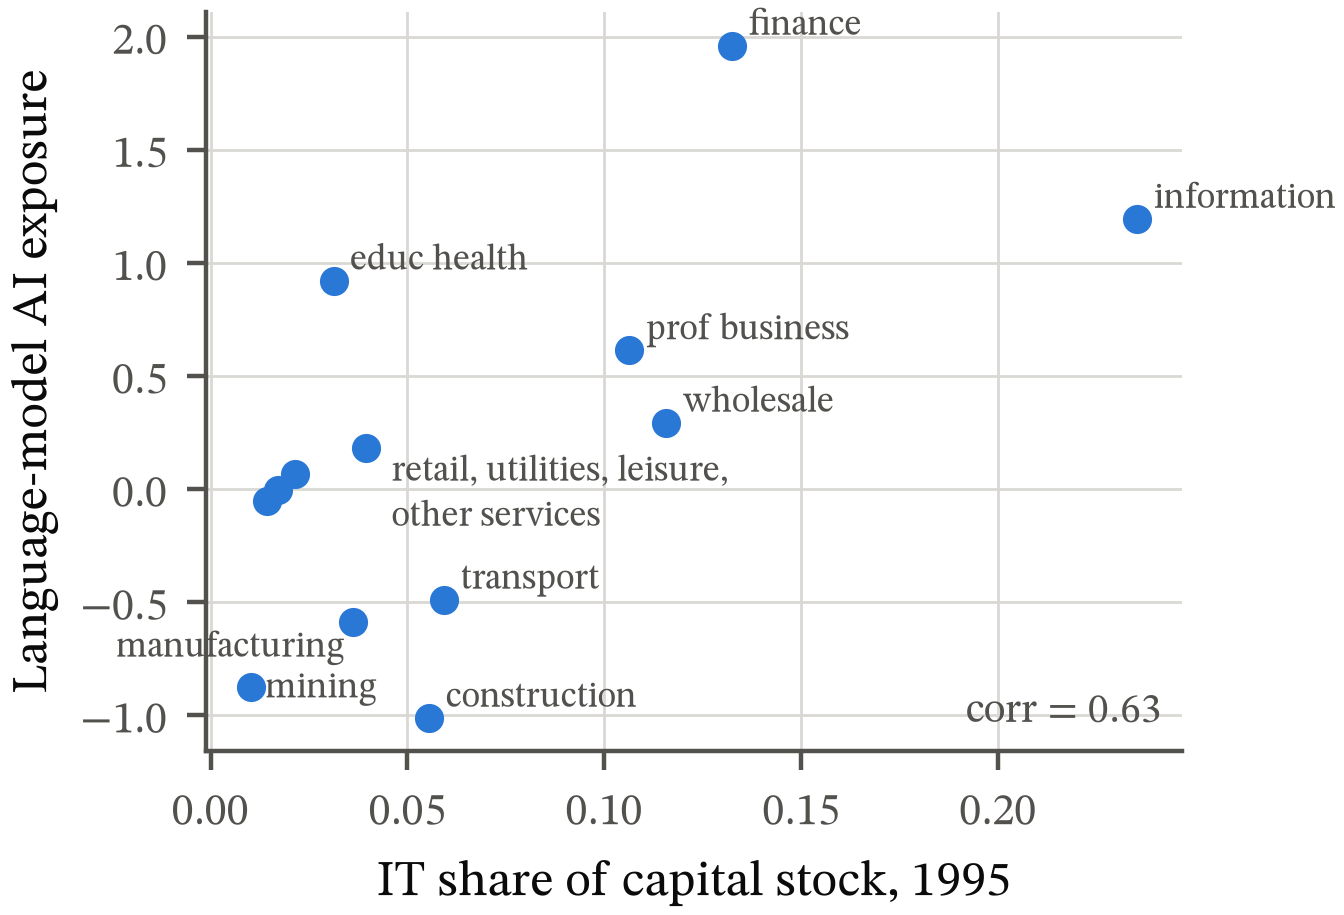
\includegraphics[width=\linewidth]{fig09_exposure_overlap.png}
    \caption{IT exposure versus AI exposure}
    \label{fig:overlap}
  \end{subfigure}
  \caption{(a) Event study of log total employment on AI exposure across 91 detailed CES industries, relative to 2019, with 95\% intervals; flat throughout. (b) Sector IT capital share in 1995 against language-model AI exposure (correlation 0.63).}
\end{figure}
